\documentclass[11pt]{article}

\usepackage{physics}
\usepackage[top=1in, bottom=1in, left=0.5in, right=0.5in]{geometry}
\usepackage{hanging}
\usepackage{amsfonts, amsmath, amssymb}
\usepackage[none]{hyphenat}
\usepackage{fancyhdr}
\usepackage[nottoc, notlot, notlof]{tocbibind}
\usepackage{graphicx}
\graphicspath{{./images/}}
\usepackage{float}
\usepackage{siunitx}
\usepackage{esint}

\pagestyle{fancy}
\fancyhead{}
\fancyfoot{}
\fancyhead[L]{MAP2302 Professor Jury}
\fancyhead[R]{Sai Sivakumar 9/16/20}
\fancyfoot[R]{\thepage}
\renewcommand{\headrulewidth}{0pt}

\setlength{\parindent}{0cm}
\setlength{\parskip}{5pt}
\renewcommand{\baselinestretch}{1.25}

\newcommand{\ihat}{\boldsymbol{\hat{\textbf{\i}}}}
\newcommand{\jhat}{\boldsymbol{\hat{\textbf{\j}}}}
\newcommand{\dr}{\vec{r}~^{\prime}(t)}
\newcommand{\dx}{x^{\prime}(t)}
\newcommand{\dy}{y^{\prime}(t)}

\newcommand{\br}[1]{\left(#1\right)}
\newcommand{\sbr}[1]{\left[#1\right]}
\newcommand{\cbr}[1]{\{#1\}}

\usepackage{mathtools}

\DeclarePairedDelimiterX{\abr}[1]{\langle}{\rangle}{#1}

\setcounter{page}{1}

\begin{document}
Section 2.2 Problems 7, 11, 13, 14, 30, 31 and Exercise from Section 1 of the Week 2 Supplement\\

7. $x\dv{y}{x} = \frac{1}{y^3}$ Solve.

No equilibria.
$$x\dv{y}{x} = \frac{1}{y^3} \to y^3\dd{y} = \frac{1}{x}\dd{x} \to \int y^3\dd{y} = \int \frac{1}{x}\dd{x} \to \frac{y^4}{4} = \ln{\abs{x}} + C$$

Hence the integral curve is of the form $$y=\br{4\ln{\abs{x}}+C}^\frac{1}{4}$$ for $x\in \mathbb{R}\setminus\cbr{0}$.\\

11. $x\dv{v}{x} = \frac{1-4v^2}{3v}$ Solve.

There are equilibrium solutions that form where $v=\pm \frac{1}{2}$.
$$x\dv{v}{x} = \frac{1-4v^2}{3v} \to \frac{3v}{1-4v^2}\dd{v} = \frac{1}{x}\dd{x} \to \int \frac{3v}{1-4v^2}\dd{v} = \int \frac{1}{x}\dd{x}$$

Let $u=1-4v^2$ and  $\dd{u} = -8v\dd{v}$.
$$-\frac{3}{8}\int \frac{1}{u}\dd{u} = \int \frac{1}{x}\dd{x} \to \ln{\abs{u}} = -\frac{8}{3}\ln{\abs{x}} + C \to \abs{1-4v^2} = C\abs{x}^{-\frac{8}{3}} \to 1-4v^2 = \pm C\abs{x}^{-\frac{8}{3}}$$

Hence the integral curve is of the form $$v=\pm\sqrt{\frac{1 \mp C\abs{x}^{-\frac{8}{3}}}{4}}$$ for $x\in \mathbb{R}\setminus\cbr{0}$.\\

13. $\dv{y}{x} = 3x^2\br{1+y^2}^{\frac{3}{2}}$ Solve.

No equilibria.
$$\dv{y}{x} = 3x^2\br{1+y^2}^{\frac{3}{2}} \to \frac{1}{\br{1+y^2}^{\frac{3}{2}}}\dd{y} = 3x^2\dd{x} \to \int \frac{1}{\br{1+y^2}^{\frac{3}{2}}}\dd{y} = \int 3x^2\dd{x}$$

Let $y=\tan{t}$ and $\dd{y} = \sec^2{t}\dd{t}$.
$$\int \frac{\sec^2{t}}{\br{1+\tan^2{t}}^{\frac{3}{2}}}\dd{t} = x^3 + C \to \int \cos{t}\dd{t} = x^3 + C \to \sin{t} = x^3 + C \to \sin{\arctan{y}} = x^3 + C$$

Using trigonometry, it is apparent that $\sin{\arctan{y}} = \frac{y}{\sqrt{1+y^2}}$.

Then:
$$\frac{y}{\sqrt{1+y^2}} = x^3 + C \to \frac{y^2}{1+y^2} = \br{x^3 + C}^2 \to y^2 = \br{x^3 + C}^2 + y^2\br{x^3 + C}^2 \to y^2\br{1-\br{x^3 + C}^2} = \br{x^3 + C}^2$$

Hence the integral curve is of the form $$y = \pm\sqrt{\frac{\br{x^3 + C}^2}{\br{1-\br{x^3 + C}^2}}}$$ for $x \in \mathbb{R}$.\\

14. $\dv{x}{t} - x^3 = x$ Solve.

There is an equilibrium solution that forms where $x=0$.
$$\dv{x}{t} - x^3 = x \to \frac{1}{x+x^3}\dd{x} = \dd{t} \to \int \frac{1}{x\br{1+x^2}}\dd{x} = \int \dd{t}$$

Let $x=\tan{u}$ and $\dd{x} = \sec^2{u}\dd{u}$. Then with a trivial substitution afterwards:
$$\int \frac{\sec^2{u}}{\tan{u}\br{1+\tan^2{u}}}\dd{u} = t + C \to \int \frac{\cos{u}}{\sin{u}}\dd{u} = t + C \to \ln\abs{\sin{u}} = t + C \to \sin{\arctan{x}} = \pm C\exp\br{t}$$

Using trigonometry, it is apparent that $\sin{\arctan{x}} = \frac{x}{\sqrt{1+x^2}}$.

Then:
$$\frac{x}{\sqrt{1+x^2}} = \pm C\exp\br{t} \to \frac{x^2}{1+x^2} = C\exp\br{2t} \to x^2 = C\exp\br{2t} + x^2C\exp\br{2t} \to x^2\br{1-C\exp\br{2t}} = C\exp\br{2t}$$

Hence the integral curve is of the form $$x = \pm\sqrt{\frac{C\exp\br{2t}}{\br{1-C\exp\br{2t}}}}$$ for $t\in \mathbb{R}$.\\

30.

(a) $\dv{y}{x} = \br{x-3}\br{y+1}^{\frac{2}{3}}$ Solve.
$$\dv{y}{x} = \br{x-3}\br{y+1}^{\frac{2}{3}} \to \br{y+1}^{-\frac{2}{3}}\dd{y} = \br{x-3}\dd{x} \to \int \br{y+1}^{-\frac{2}{3}}\dd{y} = \int \br{x-3}\dd{x} \to 3\br{y+1}^{\frac{1}{3}} = \frac{x^2}{2} - 3x + C$$

Hence the integral curve is of the form $$y = -1 + \br{\frac{x^2}{6} - x + C}^3$$ for $x\in \mathbb{R}$.

(b) Observe that $y\equiv -1 \implies \dv{\br{-1}}{x} = 0$ and $\dv{y}{x}\rvert_{y=-1} = \br{x-3}\br{\br{-1}+1}^{\frac{2}{3}} = 0$ 

(c) Note that in order to find that $y = -1$, we require $\frac{x^2}{6} - x + C = 0$ and there is no \textbf{constant} value of $C$ that can be chosen. Hence we have lost the $y = -1$ solution.

31. 

(a) $\dv{y}{x} = xy^3$ Solve.
$$\dv{y}{x} = xy^3 \to y^{-3}\dd{y} = x\dd{x} \to \int y^{-3}\dd{y} = \int x\dd{x} \to \frac{1}{-2y^2} = \frac{x^2}{2} + C$$

Hence the integral curve is of the form $$y = \pm\sqrt{\frac{1}{-x^2 + C}}$$ for $x \in \br{-\sqrt{C},\sqrt{C}}$.

(b) and (c) :

$\br{1} = \pm\sqrt{\frac{1}{-\br{0}^2 + C}} \implies C = 1 \implies y = \pm\sqrt{\frac{1}{-x^2 + 1}}$ for $x \in \br{-1,1}$.\\
$\br{\frac{1}{2}} = \pm\sqrt{\frac{1}{-\br{0}^2 + C}} \implies C = 4 \implies y = \pm\sqrt{\frac{1}{-x^2 + 4}}$ for $x \in \br{-2,2}$.\\
$\br{2} = \pm\sqrt{\frac{1}{-\br{0}^2 + C}} \implies C = \frac{1}{4} \implies y = \pm\sqrt{\frac{1}{-x^2 + \frac{1}{4}}}$ for $x \in \br{-\frac{1}{2},\frac{1}{2}}$.\\

(d) :

$\br{a} = \pm\sqrt{\frac{1}{-\br{0}^2 + C}} \implies C = \frac{1}{a^2} \implies y = \pm\sqrt{\frac{1}{-x^2 + \frac{1}{a^2}}}$ for $x \in \br{-\frac{1}{a},\frac{1}{a}}$.

If we take $\lim_{a\to 0^{+}} \frac{1}{a}$, then we find that it tends to $\infty$, and thus the domain of the integral curve is $x \in \br{-\infty,\infty}$. Likewise, if we take $\lim_{a\to \infty} \frac{1}{a}$ we find that it tends to $0$ and so the function will only be defined on $x=0$ since the adjacent real numbers cause the function to explode.\\

(e) Graphing the positive curves (red: $a=\pm \frac{1}{2}$, purple: $a=\pm 1$, black: $a=\pm 2$):

\begin{figure}[h]
\centering
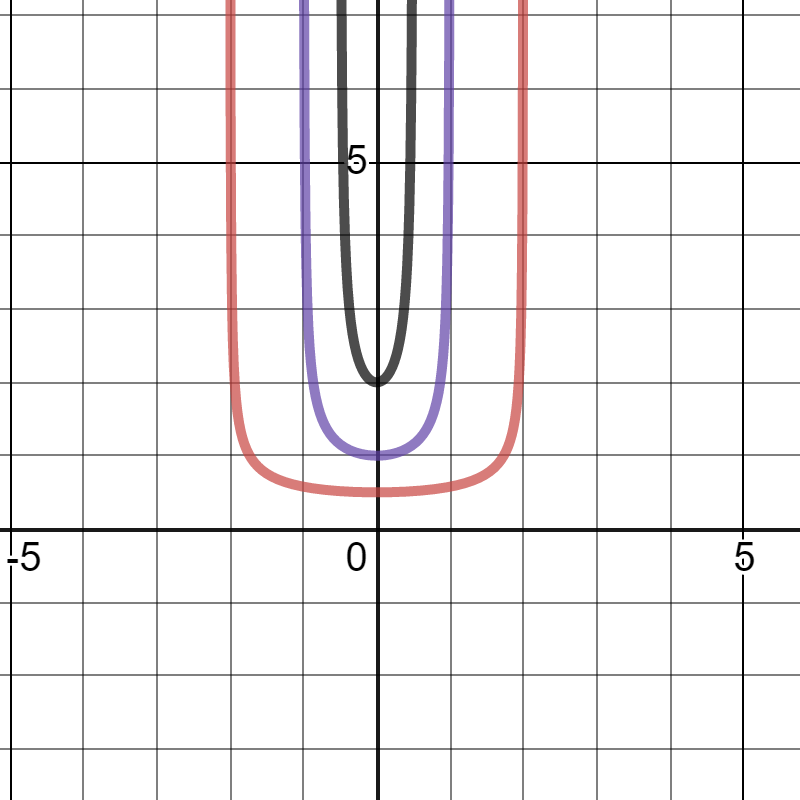
\includegraphics[scale=0.3]{plots}
\end{figure}

\newpage
Exercise from Section 1 of the Week 2 Supplement:

At every point $\br{t,x}$ on the integral curve $x = \varphi\br{t}$ all tangent vectors come in the form $\vec{w} = k\br{1,\dot{x}}$. Then the dot product of all tangent vectors $\vec{w}$ with the vector field $\vec{u}\br{t,x}$ is 0:
\begin{equation*}
\abr{\vec{u}\br{t,x}, \vec{w}} \to \abr*{\br{g(t), -\frac{1}{h(x)}}, k\br{1,g(t)h(x)}} \to k\br{g(t) + \br{-g(t)}} = 0
\end{equation*}

\end{document}